\documentclass{beamer}
\usepackage{beamerthemesplit}
\usepackage{wrapfig}
\usetheme{SPbGU}
\usepackage{pdfpages}
\usepackage{amsmath}
\usepackage{cmap} 
\usepackage[T2A]{fontenc} 
\usepackage[utf8]{inputenc}
\usepackage[english,russian]{babel}
\usepackage{indentfirst}
\usepackage{amsmath}
\usepackage{tikz}
\usepackage{multirow}
\usepackage[noend]{algpseudocode}
\usepackage{algorithm}
\usepackage{algorithmicx}
\usetikzlibrary{shapes,arrows}
\usepackage{fancyvrb}
\newtheorem{rutheorem}{Теорема}
\newtheorem{ruproof}{Доказательство}
\newtheorem{rudefinition}{Определение}
\newtheorem{rulemma}{Лемма}
\beamertemplatenavigationsymbolsempty

\title[]{Использование символьных конечных
преобразователей для лексического анализа динамически формируемого кода}

% То, что в квадратных скобках, отображается в левом нижнем углу. 
\institute[СПбГУ]{
Санкт-Петербургский государственный университет \\
Кафедра системного программирования }

% То, что в квадратных скобках, отображается в левом нижнем углу.
\author[Егор Гумин]{Егор Гумин \\
  % У научного руководителя должна быть указана научная степень
  \and  
    {\bfseries Научный руководитель:} ст.пр. С.В. Григорьев \\ 
  % Для курсовой не обязателен. Должна быть указана должность или ученая степень
  \and
    }

\date{26 мая 2016г.}

\definecolor{orange}{RGB}{179,36,31}

\begin{document}
{
% Лого университета или организации, отображается в шапке титульного листа
\begin{frame}
  \begin{center}
  {
\includegraphics[width=1.5cm]{../pictures/SPbGU_Logo.png}}
  \end{center}
  \titlepage
\end{frame}
}

\begin{frame}[fragile]
  \transwipe[direction=90]
  \frametitle{Предметная область}
  \textbf{}При обработке динамически формируемого кода возникает задача обеспечения подсветки синтаксиса и анализа ошибок\\
  \vspace{5mm}
  {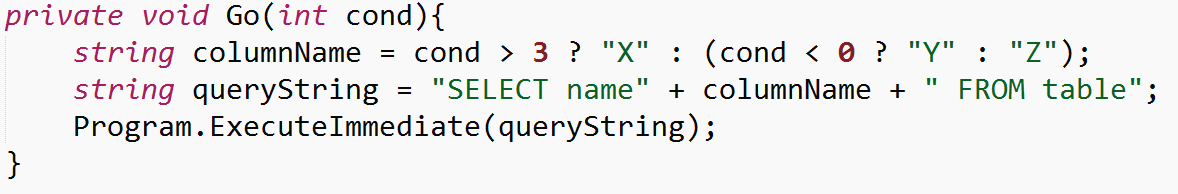
\includegraphics[width=1\linewidth]{../pictures/sql.PNG}}
  \begin{itemize}
    \item Сложности: условия, циклы, строковые операции (replace, concat)
    \item Примеры: HTML в JavaScript, SQL в C\#
    \item Необходимость: поддержка и рефакторинг существующего кода
  \end{itemize}
\end{frame}

\begin{frame}[fragile]
  \transwipe[direction=90]
  \frametitle{Лексический анализ}
  \textbf{}Задача лексического анализа — выделить лексемы во входном потоке, сохранив привязку к исходному коду \\
  \vspace{5mm}
  \textbf{}Композиция двух конечных преобразователей — основная операция при лексическом анализе: \\
    $$ComposeFST \langle symbol*position, token \rangle = \\ CodeFST\langle symbol*position, symbol\rangle \circ LexerFST \langle symbol, token\rangle$$

  \vspace{5mm}
  {}Результат композиции — FST, который можно применить к входному потоку и получить расположение в нем лексем
\end{frame}

\begin{frame}[fragile]
  \transwipe[direction=90]
  \frametitle{Реализация лексических анализаторов}
  \textbf{}Finite State Transducer (FST)
  \begin{itemize}
    \item Быстро разрастается (по количеству дуг) при большом алфавите
    \item Чаще всего не поддерживает бесконечные алфавиты
  \end{itemize}
  \vspace{5mm}
  \textbf{}Symbolic Transducer (ST)
  \begin{itemize}
    \item Каждому переходу можно сопоставить формулу (например, регулярное выражение)
    \item Возможна работа с бесконечным алфавитом
    \item Однозначность — каждому входу соответствует только один выход
  \end{itemize}
\end{frame}

\begin{frame}[fragile]
  \transwipe[direction=90]
  \frametitle{Обзор}
  \begin{itemize}
    \item YaccConstructor — исследовательский проект в области лексического и синтаксического анализа
    \item В YaccConstructor используется FST, а не ST
    \item В библиотеке Microsoft.Automata, разработанной в Microsoft Research, реализован ST, некоторые другие формализмы и операции над ними
  \end{itemize}
\end{frame}

% Обязательный слайд: четкая формулировка цели данной работы и постановка задачи
% Описание выносимых на защиту результатов, процесса или особенностей их достижения и т.д.
\begin{frame}
  \transwipe[direction=90]
  \frametitle{Постановка задачи}
  \textbf{Цель:} исследовать возможность применения ST для лексического анализа \\
  \vspace{5mm}
  \textbf{Задачи}:
  \begin{itemize}
  \item Изучить возможности библиотеки Microsoft.Automata
  \item Провести сравнение производительности алгоритма операции композиции на ST в библиотеке с производительностью операции композиции над FST в проекте YaccConstructor
  \item На основании полученных результатов сделать выводы о применимости библиотеки в проекте YaccConstructor
  \end{itemize}
\end{frame}

\begin{frame}
  \transwipe[direction=90]
  \frametitle{Изучение библиотеки}
  \begin{itemize}
    \item Разрабатывалась для решения задач формальной верификации 
    \item Активно использует SMT-решатель Z3
    \item Содержит реализацию множества формализмов (символьные автоматы, преобразователи)
    \item Для описания преобразователей широко используются языки Bek, Bex
  \end{itemize}
\end{frame}

\begin{frame}
  \transwipe[direction=90]
  \frametitle{Диаграмма решения}
  \begin{center}
  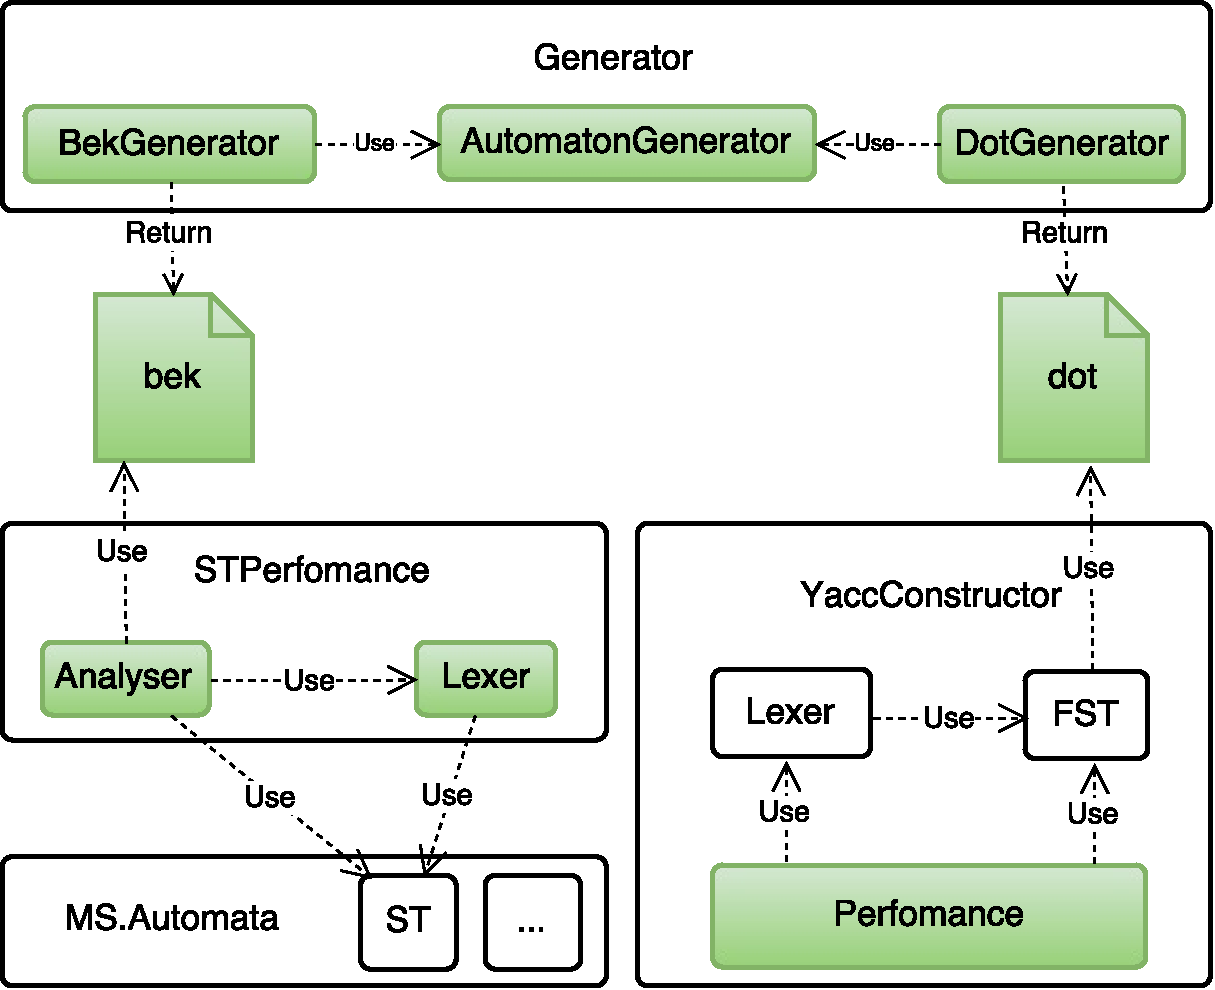
\includegraphics[width=0.8\textwidth]{../pictures/YC.pdf}
  \end{center}
\end{frame}


\begin{frame}
  \transwipe[direction=90]
  \frametitle{Результаты эксперимента}
    
\begin{table}[H]
\begin{center}
\begin{tabular}{c c}
\begin{minipage}{0.4\textwidth}
\begin{tabular}{|c|c|c|}

\hline 
Тест & Ребра & Вершины\\  
\hline 
1 & 1 & 2 \\
2 & 6 & 5 \\
3 & 25 & 20 \\
4 & 50 & 5 \\
5 & 60 & 50 \\
\hline 

\end{tabular}
\end{minipage}
&
\begin{minipage}{0.6\textwidth}
 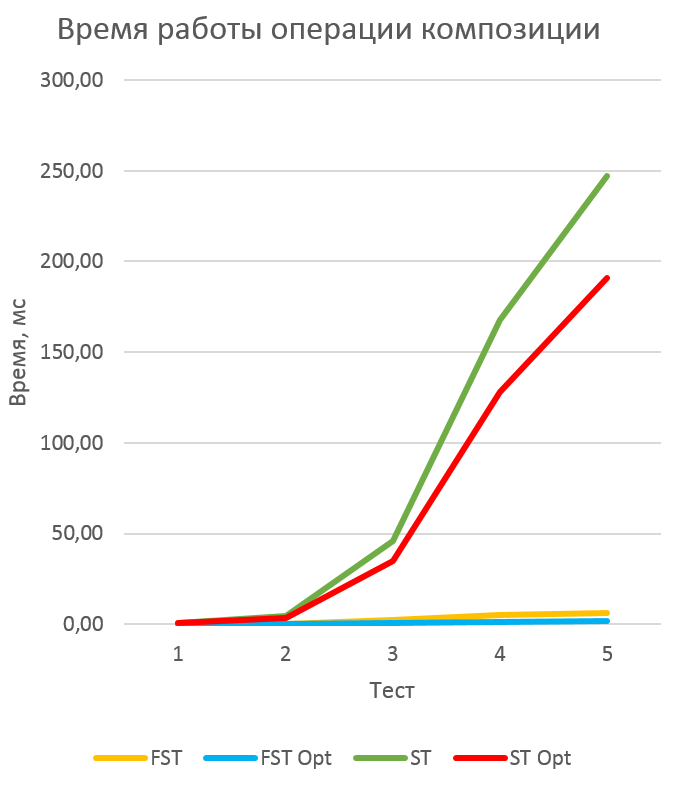
\includegraphics[width=0.9\textwidth]{../pictures/newgraph1.PNG}
\end{minipage}

\end{tabular}

\end{center}
\end{table} 
\end{frame}


\begin{frame}
  \transwipe[direction=90]
  \frametitle{Выводы}
  \begin{itemize}
    \item ST применимы для лексического анализа
    \item Библиотека Microsoft.Automata разрабатывалась для решения задач формальной верификации и не обладает необходимой производительностью
    \item Необходима реализация ST, адаптированная под задачи проекта YaccConstructor
  \end{itemize}
\end{frame}



\begin{frame}
  \transwipe[direction=90]
  \frametitle{Результаты}
  \begin{itemize}
    \item Исследованы возможности библиотеки Microsoft.Automata
    \item Проведено сравнение производительности алгоритма операции композиции на ST в библиотеке с производительностью операции композиции над FST в проекте YaccConstructor
    \item На основании полученных результатов сделаны выводы о необходимости написания собственной реализации ST
    \item Сделан доклад на конференции «Современные технологии в теории и практике программирования», публикация в сборнике конференции
  \end{itemize}
\end{frame}


\end{document}
